\section{Auswertung}
\label{sec:Auswertung}

\subsection{Charakteristik des Geiger-Müller-Zählrohrs}

In \autoref{fig:plot1} wird die Impulsrate $N$
gegen die Betriebsspannung $U$ aufgetragen.
Bei einer Integrationszeit von $\increment t = \qty{120}{\second}$ ergibt sich für die Impulsrate
und für den Fehler der Poisson-Verteilung der Impulse $n$
\begin{align} \label{eq:impulsrate}
    N = \frac{n \pm \increment n}{\increment t} = N' + \increment N
    \quad \text{mit} \quad
    \increment n = \sqrt{n} \, .
\end{align}

\begin{figure}
    \centering
    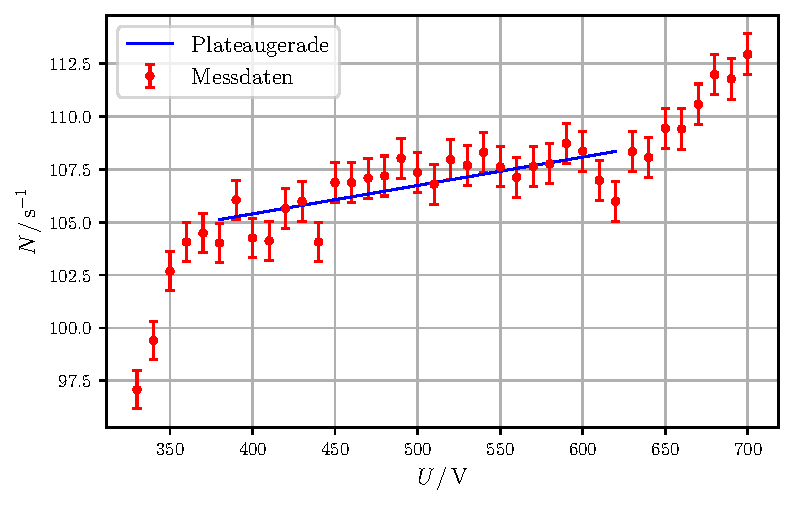
\includegraphics[width = 0.9\linewidth]{build/plot1.pdf}
    \caption{Die Impulsrate $N \mathbin{/} \mathrm{s^{-1}}$ pro Spannung $U$.
    Die lineare Ausgleichsgerade, liegt im Plateaubereich bei einer Spannung
    von $\qty{380}{\volt} - \qty{620}{.\volt}$.}
    \label{fig:plot1}
\end{figure}

Für die Ausgleichsgerade des Plateaubereichs mit der Geradengleichung
\begin{equation*}
    N = a \cdot U + b 
\end{equation*}
ergeben sich die Parameter
\begin{align*}
    a &= \qty{0.013(3)}{\per\volt} \quad \text{und} \\
    b &= \num{100.02(142)} \, .
\end{align*}

Für die Güte des Geiger-Müller-Zählrohrs ergibt sich aus der Plateau-Steigung $M$ in in
$\mathrm{percent}$ pro $\qty{100}{V}$
\begin{equation*}
    M = 1 - \frac{a \cdot \qty{400}{V}}{a \cdot \qty{500}{V}} 
    = \qty{1.26(25)}{\percent} \; \text{pro} \; \qty{100}{V} 
\end{equation*}


\subsection{Bestimmung der Nachentladungszeit}

Um den zeitlichen Abstand zwischen Primär- und Nachentladungsimpulsen zu bestimmen,
werden die Impulse auf einem Oszilloskop wie in \autoref{fig:osz} zu erkennen dargestellt.
\begin{figure}
    \centering
    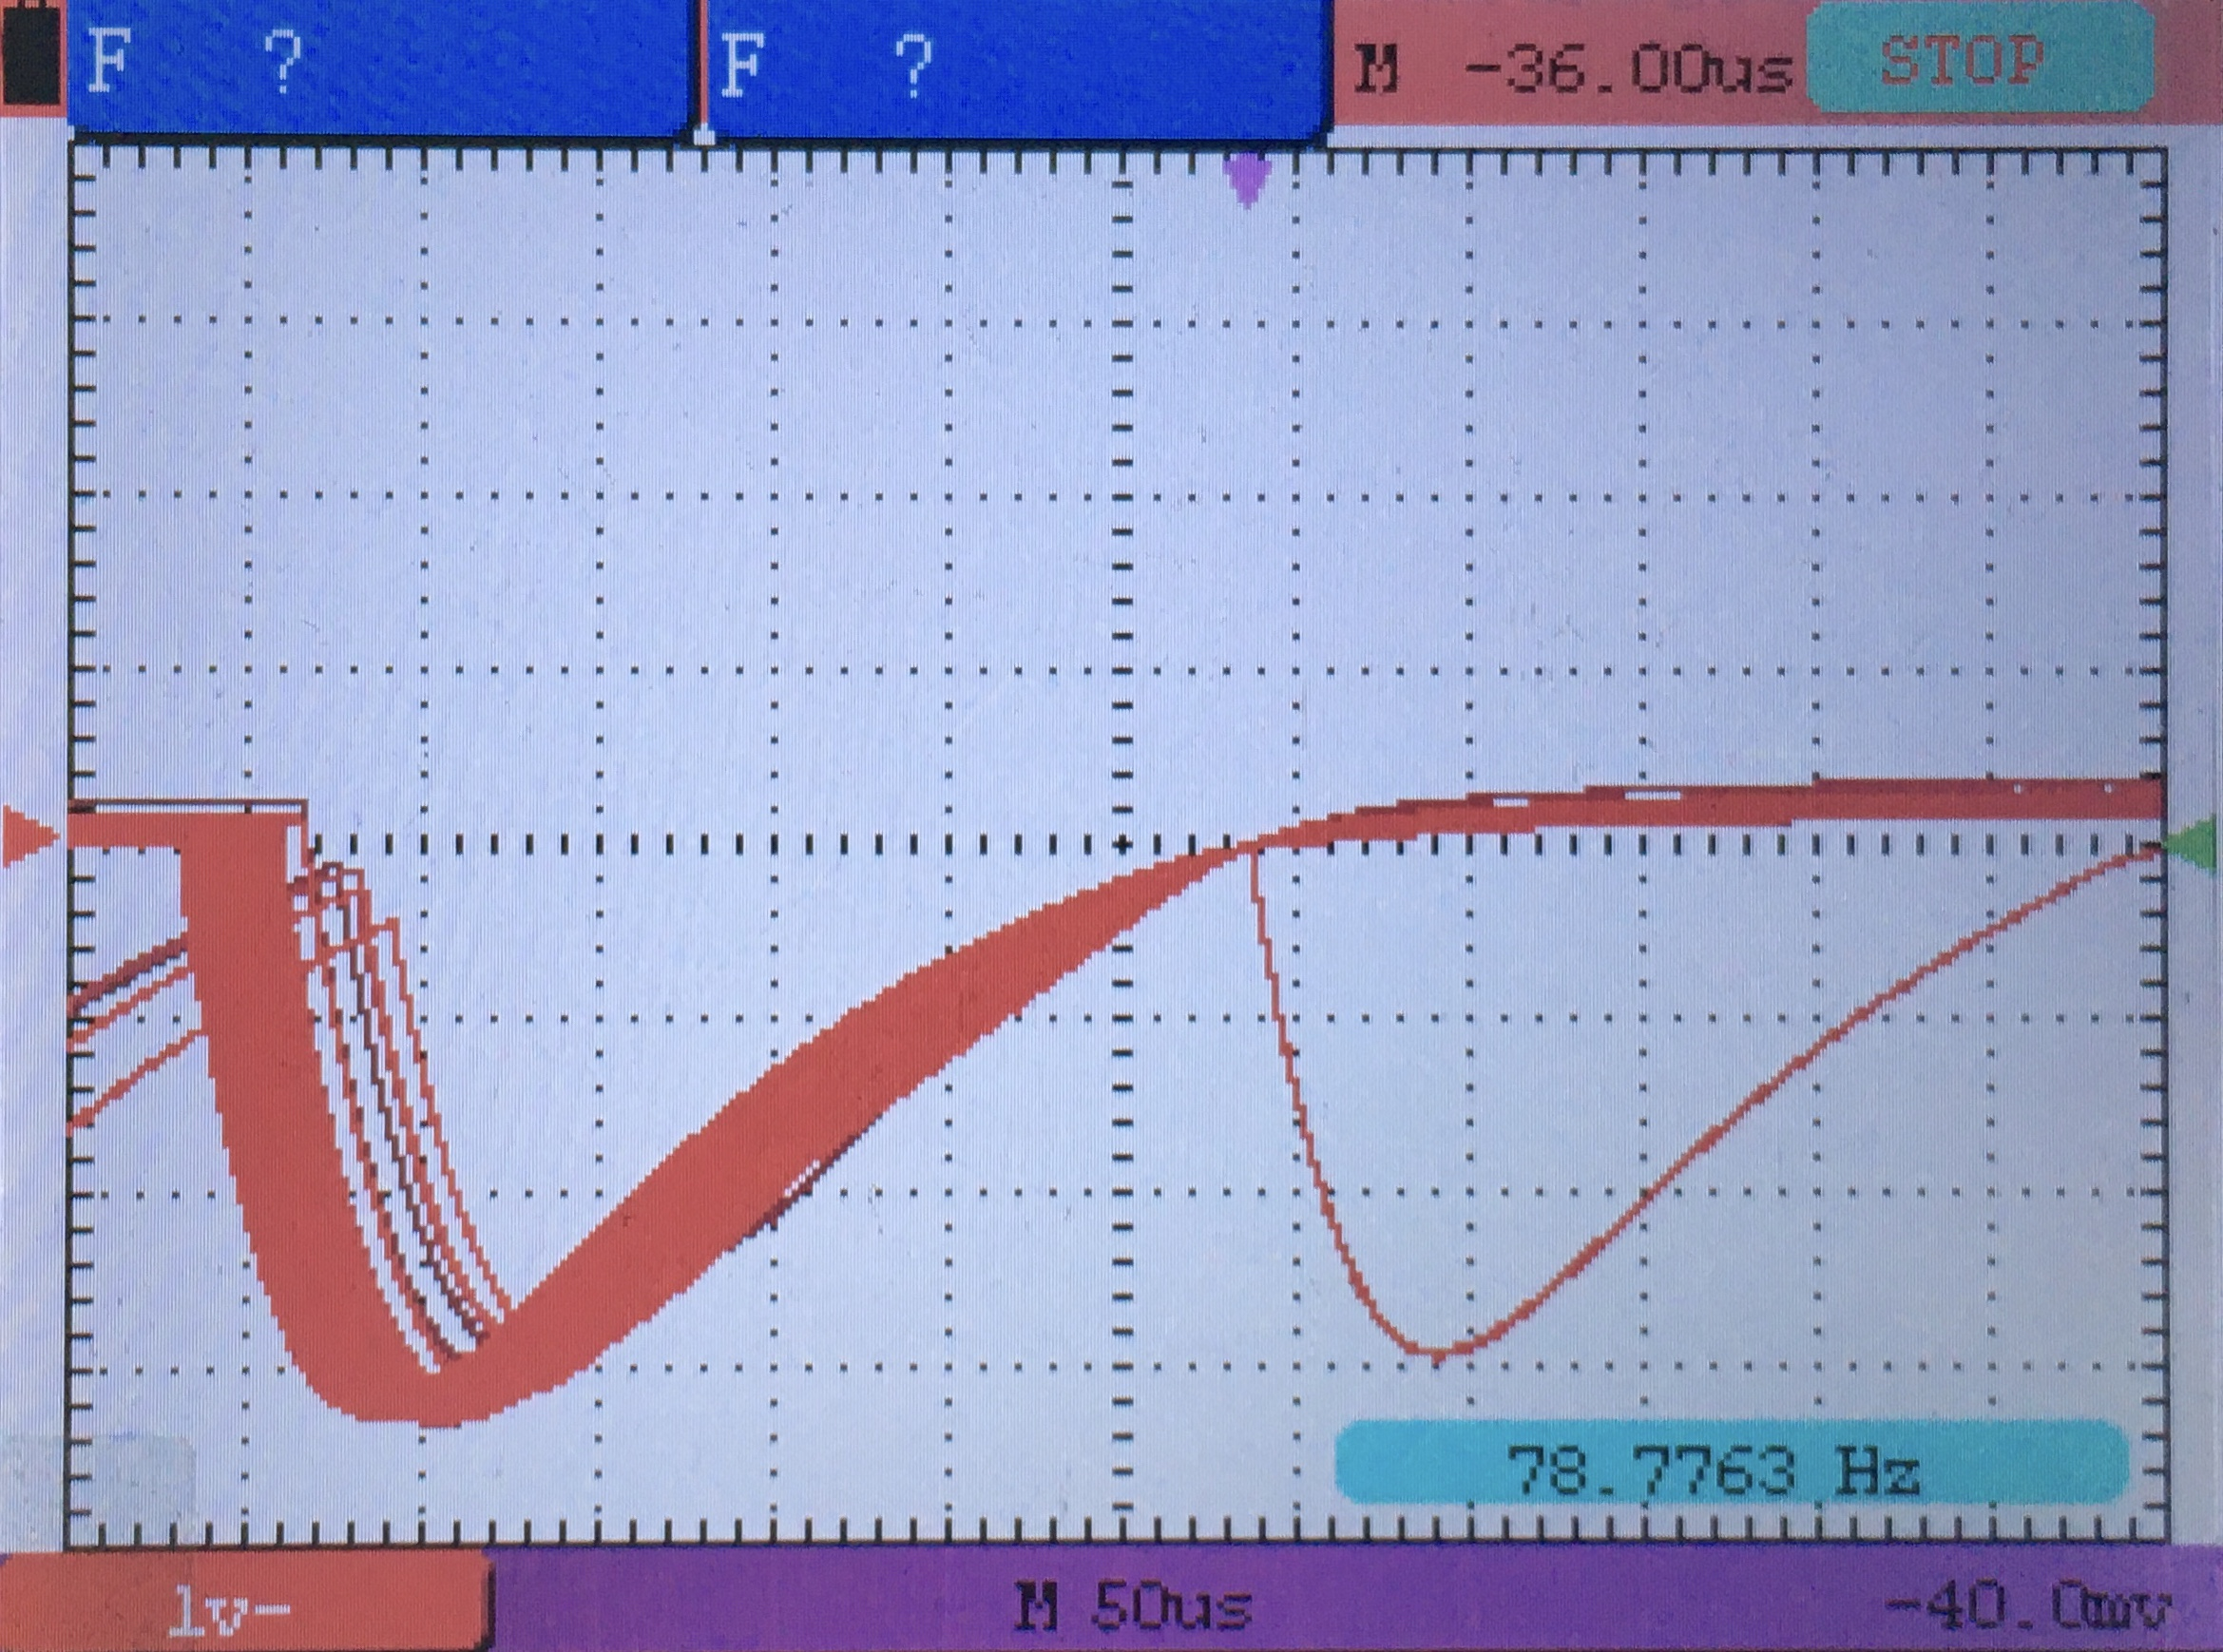
\includegraphics[width = 0.8\linewidth]{pictures/osz.jpg}
    \caption{Primär und Nachentladungen bei $U = \qty{700}{V}$.}
    \label{fig:osz}
\end{figure}

Dafür wird die Spannung soweit verringert, bis kein weiterer Impuls zu sehen ist.
Nachdem die Spannung auf $\qty{700}{V}$ erhöht wird, werden Nachentladungen in Form von Impulsen sichtbar.
Die Nachentladungszeit wird von Peak zu Peak abgelesen und ergibt ungefähr
\begin{equation*}
    T_\text{Nachentladung} \approx 5,8 \cdot \qty{50}{\micro\second} = \qty{290}{\micro\second} \, .
\end{equation*}


\subsection{Bestimmung der Totzeit}

\subsubsection*{Zwei-Quellen-Methode}

Für die Zwei-Quellen-Methode ergeben sich die Impulsraten nach \autoref{eq:impulsrate} zu
\begin{align*}
    N_{1}   =\frac{1334 \pm 37}{120 \mathrm{s}}, \quad 
    N_{2}   =\frac{21994 \pm 148}{120 \mathrm{s}}, \quad 
    N_{1+2} =\frac{23182 \pm 152}{120 \mathrm{s}}
\end{align*}
damit ergibt sich nach \autoref{eq:T_Tot} die Totzeit zu
\begin{equation}
    T_\text{Quell} \approx \qty{300(400)}{\micro\second}
\end{equation}
mit dem Fehler nach \autoref{eq:fehlerfortplanzung}
\begin{equation*}
    \increment T  = \sqrt{
      \left(\frac{N_{1+2}-N_{2}}{2 N_{1}^{2} N_{2}} \cdot \increment N_{1}\right)^{2} 
    + \left(\frac{N_{1+2}-N_{1}}{2 N_{1} N_{2}^{2}} \cdot \increment N_{2}\right)^{2} 
    + \left(-\frac{1}{2 N_{1} N_{2}} \cdot \increment N_{1+2}\right)^{2}
    } \, .
\end{equation*}

\subsubsection*{Oszilloskop-Methode}

In \autoref{fig:osz} kann neben der Nachentladungszeit auch die Totzeit abgelesen werden, 
indem wie in \autoref{fig:Diagramm2} dargestellt der zeitliche Abstand zwischen Peak und Aufstieg
des nächsten Impulses abgelesen. Für die Totzeit ergibt sich daraus
\begin{equation*}
    T_\text{Osz} \approx 4,8 \cdot \qty{50}{\micro\second} = \qty{240}{\micro\second} \, .
\end{equation*}


\subsection{Freigesetzte Ladungen}

Nach \autoref{eq:ladungen} werden die freigesetzten Ladungen pro einfallendem Teilchen berechnet.
Auch hier ergibt sich ein Fehler der einfallen Teilchen $Z$ nach \autoref{eq:fehlerfortplanzung}
\begin{equation*}
    \increment Z 
    = \sqrt{\left(\frac{1}{e N} \cdot \Delta I\right)^{2}+\left(\frac{1}{e N 2} \cdot \Delta N\right)^{2}} \, ,
\end{equation*}
wobei der Fehler des gemessenen Strom bei $\increment I = \qty{0.05}{\micro\ampere}$ liegt.

In \autoref{fig:plot2} werden die berechneten freigesetzten Ladungen graphisch dargestellt und
aus der der Vielzahl an Messdaten in \autoref{tab:ladungen} für zehn Werte tabellarisch aufgetragen.
\begin{table}
    \centering
    \caption{Die aus den Anodenströmen und Impulsraten resultierenden freigesetzten Ladungen für zehn exemplarische Werte.}
    \label{tab:ladungen}
    \begin{tabular}{c c c}
        \toprule
        $\mathrm{I} \mathbin{/} \unit{\micro\ampere}$ &
        $N \mathbin{/} \mathrm{s^{-1}}$ &
        $Z \mathbin{/} e \cdot 10^{-19}$ \\
        \midrule
        0,20 $\pm$ 0,05 & 0,856 $\pm$ 0,008 & 1,22 $\pm$ 0,30 \\
        0,35 $\pm$ 0,05 & 0,869 $\pm$ 0,008 & 2,10 $\pm$ 0,30 \\
        0,41 $\pm$ 0,05 & 0,867 $\pm$ 0,008 & 2,46 $\pm$ 0,30 \\
        0,50 $\pm$ 0,05 & 0,891 $\pm$ 0,008 & 2,92 $\pm$ 0,29 \\
        0,60 $\pm$ 0,05 & 0,900 $\pm$ 0,008 & 3,47 $\pm$ 0,29 \\
        0,70 $\pm$ 0,05 & 0,902 $\pm$ 0,008 & 4,03 $\pm$ 0,29 \\
        0,80 $\pm$ 0,05 & 0,898 $\pm$ 0,008 & 4,63 $\pm$ 0,29 \\
        0,90 $\pm$ 0,05 & 0,903 $\pm$ 0,008 & 5,18 $\pm$ 0,29 \\
        1,00 $\pm$ 0,05 & 0,912 $\pm$ 0,008 & 5,70 $\pm$ 0,29 \\
        1,15 $\pm$ 0,05 & 0,941 $\pm$ 0,008 & 6,36 $\pm$ 0,28 \\
        \bottomrule
    \end{tabular}
\end{table}

\begin{figure}
    \centering
    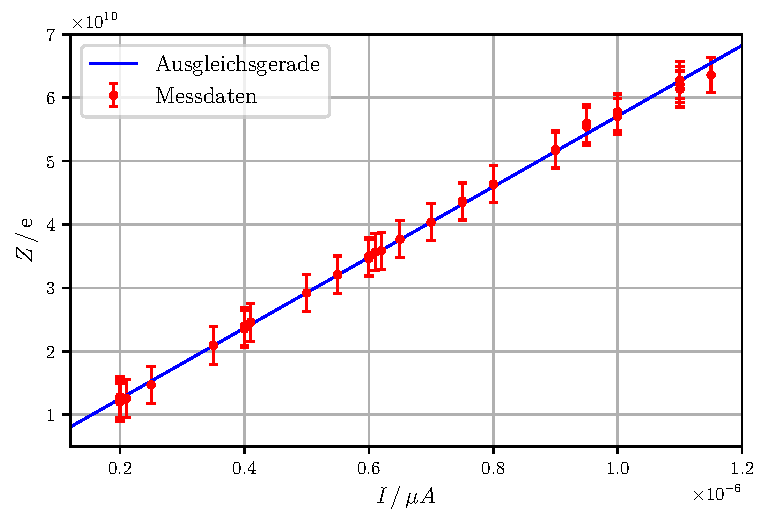
\includegraphics[width = 0.9\linewidth]{build/plot2.pdf}
    \caption{Die freigesetzten Ladungen $Z$ pro Zählerstrom $I$.}
    \label{fig:plot2}
\end{figure}